\subsection{Blockchain}
\label{sec:sota_blockchain}
    Eine Blockchain ist in ihrer Essenz ein Konzept einer immer länger werdenden, unveränderbaren, öffentlichen Kette von Transaktionen, die dezentral gespeichert wird (s. \fref{fig:bc_highlvl}). 
    \smallskip
    \begin{figure}[H]
    	\centering
    	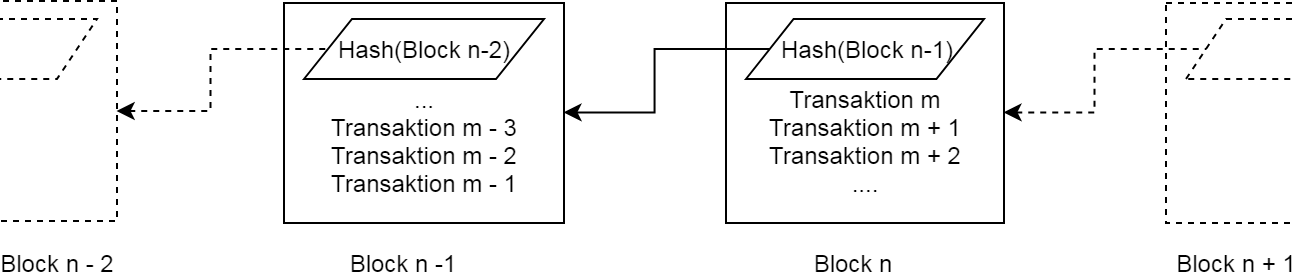
\includegraphics[width=\textwidth]{graphics/bc_highlvl.png}
    	\caption[Abstrakte Darstellung einer Blockchain]{Abstrakte Darstellung einer Blockchain. Jeder neu hinzugefügte Block (hier immer rechts angehängt) enthält mit dem Hashwert des vorigen Blocks eine Referenz auf diesen.}
    	\label{fig:bc_highlvl}
    \end{figure}
    \noindent Erstmals 2008 von Satoshi Nakamoto, ursprünglich als \gls{p2p} Electronic Cash System ,,Bitcoin``
    \!\footnote{Heute werden Bitcoin, Ether, Ripple und andere als digitale Zahlungsmittel als sogennante Kryptowährung bezeichnet} 
    erfunden, erregte die Technologie aufgrund ihrer Eigenschaften wie ihres dezentralen, anonymen Konzepts schnell Aufmerksamkeit\cite{Underwood2016}.
    Bitcoin ist die erste populäre digitale Währung, die ohne zentrale Autorität wie beispielsweise einer \gls{ttp} das in \fref{sec:sota_doublespend} vorgestellte Double-Spending Problem lösen sollte\cite{Nakamoto2008}. 
    Übertragen auf Bitcoin bedeutet es, dass ein Empfänger einer Transaktion sichergehen können muss, dass der vorige Besitzer den Bitcoin oder den Bruchteil dessen vorher nicht schon einmal erfolgreich an einen anderen Empfänger gesendet hat.
    Dies wird mittels kryptographischem Beweis, welcher in \fref{sec:sota_blockchain_consensus} genauer betrachtet wird, anstatt des laut \citeauthor{Nakamoto2008} vorstellten mangelhaften Modells der \gls{ttp}, welche stets einen Single Point of Failure
    \!\footnote{Ein Single Point of Failure stellt beipsielsweise eine Bank im Zahlungsverkehr dar.
    Fällt die Bank beispsielsweise aus irgendeinem Grund aus oder wird kompromittiert, haben deren Kunden keine Möglichkeit mehr (sicher) Überweisungen auszuführen und zu empfangen.}
    darstellt, gelöst. 
    Das Konzept ermöglicht es somit zwei Entitäten, auch, wenn diese sich gegenseitig nicht vertrauen, ohne vermittelnde Person oder Organisation sichere (im Sinne der Integrität) direkte Transaktionen  durchzuführen, welche auch im Nachhinein nicht mehr verändert werden können.\cite{Christidis2016}
    
    \subsubsection{Einführung in das Konzept}
    \label{sec:sota_blockchain_introduction}
    Grundlegend ist die Blockchain eine verteilte Datenstruktur, die zwischen den Mitgliedern eines Netzwerkes repliziert und geteilt wird.
    Die Blockchain beinhaltet das maßgebliche ,,Hauptbuch`` (im Englischen ,,Ledger`` genannt) mit allen vergangenen Transaktionen, ein Log, dessen Einträge mit Zeitstempeln jeweils zu unterschiedlichen Blöcken zusammengefasst werden.\cite{Christidis2016}
    Alle vergangenen Transaktionen sind in der Reihenfolge ihres Auftretens für alle Teilnehmer einsehbar\cite{Nakamoto2008}.
    \medskip\\
    Die Knoten des Netzwerkes speichern stets eine eigene Kopie der Blockchain.
    Da das Netzwerk ein \gls{p2p}-Netzwerk \!\footnote{In einem \gls{p2p} sind die Teilnehmer (,,Peers`` genannt) über das Internet direkt miteinander verbunden und nehmen innerhalb des Netzwerkes die Rolle des Clients, sowie des Servers ein. So können beispielsweise Dateien ohne zentralen Fileserver im Netzwerk geteilt werden.} ist, müssen nicht immer alle Knoten online sein, damit der aktuelle Stand der Blockchain verfügbar ist.\cite{Christidis2016}
    \medskip\\
    Nutzer nehmen an dem Netzwerk über die jeweiligen Knoten teil, wobei ein Knoten auch für mehrere Nutzer einen Zugang bieten kann (s. \fref{fig:bc_network}). 
    Jeder Nutzer interagiert mit dem Netzwerk mittels eines Paares von öffentlichem und privatem Schlüssel, wobei der Öffentliche direkt oder über dessen Hashwert zur Adressierung des Nutzers verwendet wird.
    Mit dem privaten Schlüssel werden die Transaktionenn des Nutzers signiert.\cite{Christidis2016}
    \medskip\\
    Zunächst wurde lediglich mit digitalen Coins gehandelt, welche einer in Form einer Kette digitaler Signaturen modelliert werden\cite{Nakamoto2008}.
    In anderen Anwendungsbereichen außerhalb der Kryptowährungen wird nicht von Coins, sondern von generalisierten Assets gesprochen.
    Der aktuelle Zustand (,,World View`` genannt) ergibt sich durch das Zurückverfolgen der einzelnen Transaktionen in der Blockchain. 
    Es wird also kein aktueller Stand, welcher Teilnehmer des Netzwerks was und wie viel besitzt, gespeichert.\cite{Christidis2016}
    \begin{figure}[H]
    	\centering
    	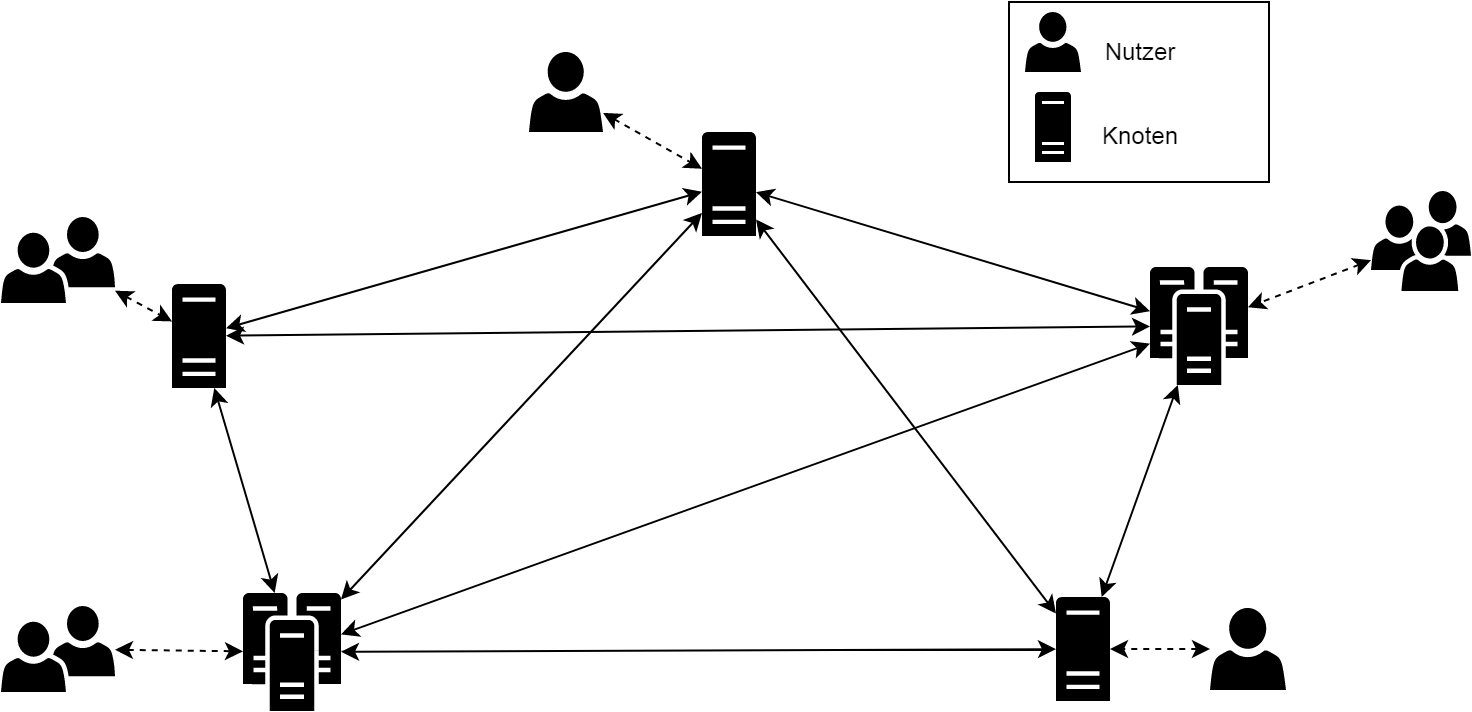
\includegraphics[width=\textwidth]{graphics/BCNetwork.png}
    	\caption[Blockchain-Netzwerk]{Blockchain-Netzwerk}
    	\label{fig:bc_network}
    \end{figure}
    
    \subsubsection{Transaktionen}
    \label{sec:sota_blockchain_trx}
    In einer Blockchain werden Aktivitäten von Nutzern in Form von Transaktionen repräsentiert.
    Tätigt ein Nutzer eine Transaktion\colorbox{light-gray}{\lstinline{X}}, so signiert er diese mit seinem privaten Schlüssel.
    Der Knoten, über welchen der Nutzer mit dem Netzwerk interagiert, validiert die Transaktion und fügt sie zu seiner Sammlung von Transaktionen für einen neuen Block hinzu.
    Zudem verbreitet der Knoten die valide Transaktion an dessen nächste Nachbarn
    \!\footnote{Nächste Nachbarn sind jene Knoten, die einen Sprung im \gls{p2p}-Netzwerk voneinander entfernt sind.}.
    Die Nachbarn überprüfen die Transaktion ebenfalls auf deren Validität und verbreiten diese wiederrum an ihre nächsten Nachbarn. 
    Schlussendlich kennen eine Vielzahl von Knoten im Netzwerk die Transaktion \colorbox{light-gray}{\lstinline{X}}. 
    Dieses zur Verbreitung der Tansaktionen verwendete Protokoll wird als ,,Gossip-Protokoll`` bezeichnet.\cite{Christidis2016}
    \medskip\\
    Im sogenannten ,,Mining``-Prozess, der für jeden neuen Block wiederholt wird, werden valide Transaktionen, die innerhalb eines im Voraus abgestimmten Zeitintervalls gesammelt wurden, zeitlich geordnet und zu einem mit Zeitstempel versehenem ,,Candidate``-Block zusammengefügt.
    Dieser wird wieder im Netzwerk verbreitet. 
    Andere Knoten im Netzwerk stellen sicher, dass der neue Block valide Transaktionen enthält und den richtigen Hash des vorigen Blocks in der Kette enthält. 
    Bei erfolgreicher Validierung hängen die Knoten den Block jeweils an ihre Kopie der Kette an, übernehmen die darin enhaltenen Transaktionen und aktualisieren somit den aktuellen Zustand. 
    Sollte innerhalb des Mining-Prozesses eine Validierung fehlschlagen, wird der ganze Block verworfen.\cite{Christidis2016}\\
    Der Knoten, der diesen Prozess ausführt, wird ,,Miner`` genannt.
    Welcher Knoten zum Miner wird ist vom genutzten Konsensmechanismus abhängig und ist unter Umständen in der gleichen Situation unterschiedlich.\cite{Christidis2016}
    \newpage
    \begin{figure}[H]
    	\centering
    	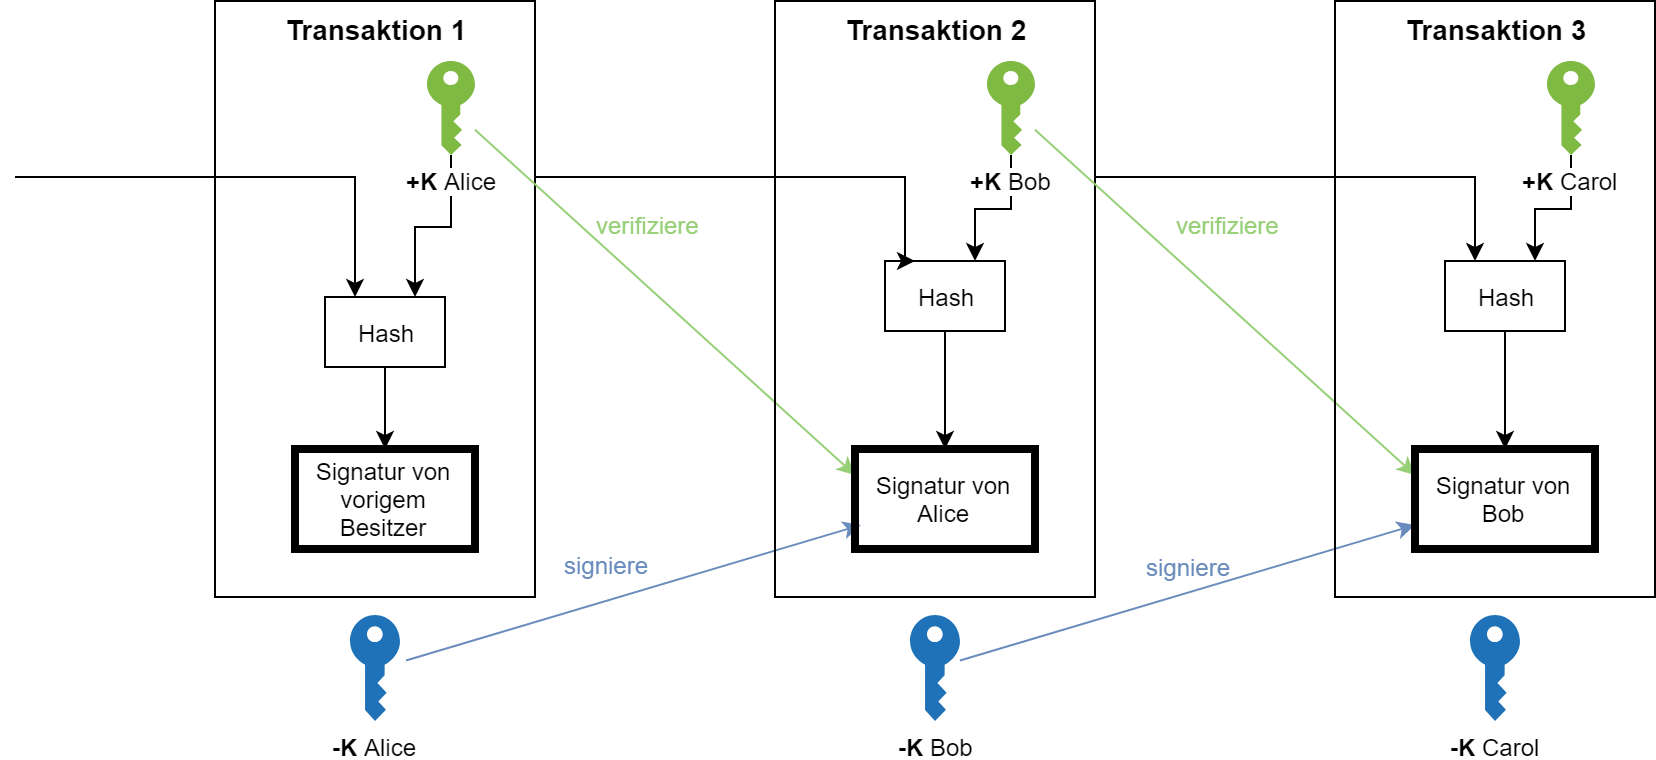
\includegraphics[width=\textwidth]{graphics/transaction.png}
    	\caption[Kette digitaler Signaturen]{Kette digitaler Signaturen\cite{Nakamoto2008}. \lstinline{+K} stellt dabei den öffentlichen und \lstinline{-K} den privaten Schlüssel dar.}
    	\label{fig:txio}
    \end{figure}
    Wie in \fref{fig:txio} dargestellt, werden Coins oder Assets von einem Sender zu einem Empfänger übertragen, in dem der Sender einen Hash der vorigen Transaktion und den öffentlichen Schlüssel des Empfängers mit seinem eigenen privaten Schlüssel digital signiert und diesen Hash dann am Ende der Transaktionskette anfügt.
    Der Empfänger, sowie alle Teilnehmer des Netzwerkes können den Besitz des Assets über die Kette der digitalen Signaturen zurückverfolgen.
    Transaktionen können zudem mehrere Ein- und Ausgaben haben.\cite{Nakamoto2008}
    
    \subsubsection{Konsens und Sicherheit}
    \label{sec:sota_blockchain_consensus}
        Um Transaktionen zu validieren, deren Reihenfolge im nächsten Block zu bestimmen und Mining-Blöcke auszuwählen zu können, wird von allen Teilnehmern des Netzwerkes ein gemeinsamer Konsens vorausgesetzt. 
        Ist dies nicht der Fall können, wie in \fref{fig:bc_forks} dargestellt, unterschiedliche Ketten (,,Forks`` genannt) innerhalb der jeweiligen Kopien der Blockchain auf den einzelnen Knoten entsehen. 
        \noindent
        \begin{figure}[H]
        	\centering
        	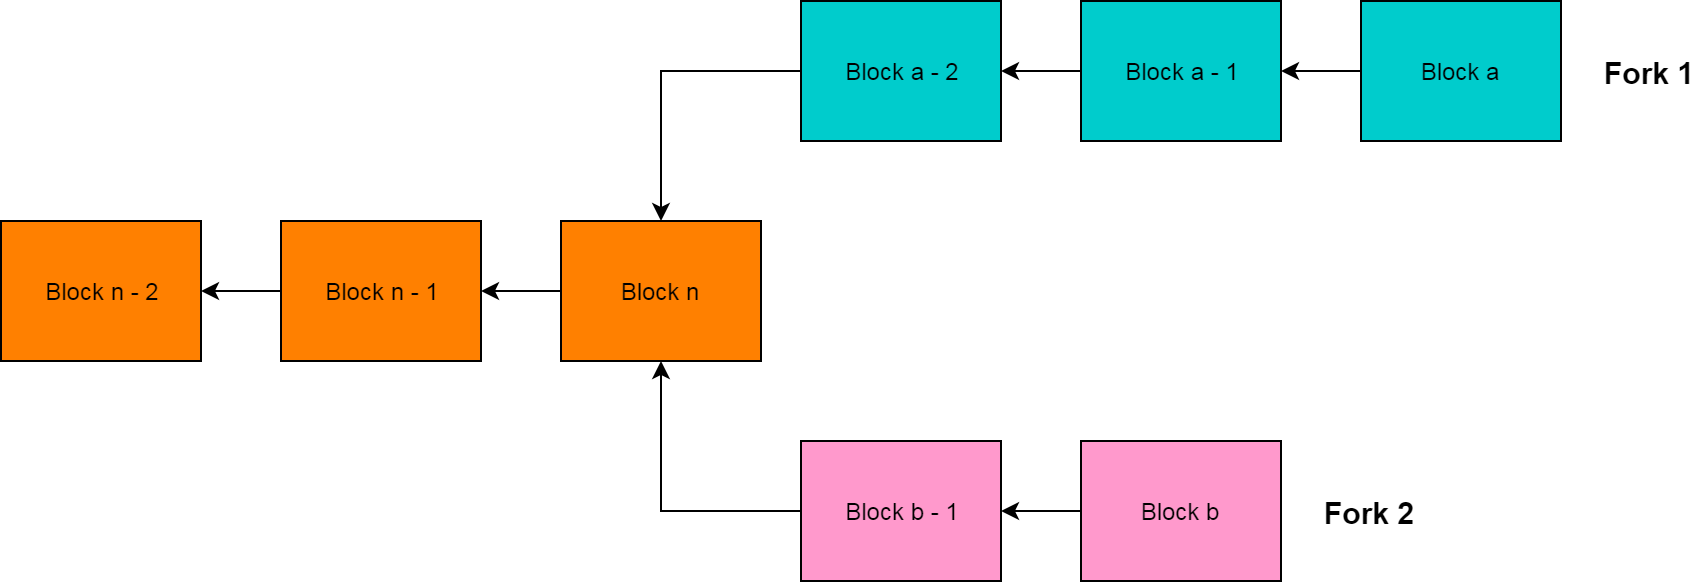
\includegraphics[width=\textwidth]{graphics/BCForks.png}
        	\caption[Blockchain mit Forks]{Blockchain mit zwei Forks}
        	\label{fig:bc_forks}
        \end{figure}
        \noindent Im Idealfall stimmen alle validierenden Knoten des Netzwerkes über eine Mehrheitsentscheidung die Reihenflolge der Transaktionen für den nächsten Block ab.\cite{Christidis2016} 
        Aufgrund der Gefahr eines ,,Sybil-Angriffs``\cite{Trifa2014}
        \!\footnote{Bei einem ,,Sybil-Angriff`` erlangt ein Angreifer mehr Einfluss auf die Abstimmung, indem er entweder zusätzliche Nutzeridentitäten für sich selbst erstellt oder mehrere Knoten kontrolliert.
        } ist dies jedoch unzumutbar.
        Um diese Gefahr zu umgehen werden unterschiedliche Methoden angewendet, von denen drei im Folgenden erläutert werden\cite{Christidis2016}.
        \medskip\\
        Bei Bitcoin wird ein sogenannnter \gls{pow} verwendet. 
        Das Mining neuer Blöcke wird rechnerisch ,,teuer`` gemacht, indem vorausgesetzt wird, dass ein minender Knoten eine richtige Zufallszahl (genannt ,,Nonce``) mit variablem Schwierigkeitsgrad, mit bestimmten Eigenschaften berechnet und mit einer bestimmten Anzahl Bitcoins belohnt wird. 
        Da bei der Berechnung kryptographische Hashfunktionen verwendet werden, kann das Ergebnis durch die anderen Knoten einfach verifiziert werden. 
        Den Nonce kann jeder Knoten im Netzwerk berechnen, sodass die explizite Auswahl des Miners entfällt. 
        Der Candidate-Block jenes Knotens, der den Nonce findet, wird an die Blockchain angehängt. 
        Versucht ein Angreifer Transaktionen zu manipulieren benötigt er mehr Rechenleistung als die legitimen Knoten im Netzwerk, um als erster mit seinem Knoten den richtigen Nonce zu finden. 
        So wird sichergestellt, dass vergangene Transaktionen auch nicht mehr rückgängig gemacht werden können.
        Sollten Forks entstehen, wird der Fork verwendet, in dem der meiste Rechenaufwand steckt.
        Dies ist entweder der längste Fork oder der Fork, mit dem höchsten Schwierigkeitsgrad.\cite{Christidis2016,Nakamoto2008}
        \medskip\\
        Alternativ kann ein \gls{pos} verwendet werden, welcher bedeutend weniger Rechenaufwand erfordert und somit engergieeffizienter ist. 
        Dabei sendet sich ein Besitzer selbst eine bestimmte Anzahl an Coins und addiert einen vordefinieren Prozentsatz als Belohnung. 
        Es werden also von den Knoten Coins eingesetzt, um einen Block Minen zu dürfen.
        Analog zum \gls{pow} wird ein Hashwert, der entweder größer oder kleiner als ein gesuchter Wert ist, berechnet.
        Der Schwierigkeitsgrad der Berechnung wird umgekehrt proportional zum Alter der Coins individuell festgelegt. 
        Der Hashwert wird aus statischen Daten, ausgenommen des Zeitstempels, berechnet, sodass bei jeder Änderung des Zeitstempels eine Chance zum Finden des Hashwertes besteht und die individuelle Rechenleistung der Knoten nur eine minimale Rolle spielt. 
        Wird ein Wert gefunden, so wird die Belohnung an den minenden Knoten ausgeschüttet und das Alter der Coins zurückgesetzt.\cite{Tschorsch2016}
        \medskip\\
        \gls{pow} und \gls{pos} werden vornehmlich in öffentlichen Netzwerken eingesetzt.
        Für private Blockchains sind sie jedoch eher ungeeignet, da in solchen Netzwerken die Teilnehmer häufig per Whitelist bekannt sind. 
        In solchen Fällen werden Algorithmen wie das Practical \gls{bft} angewendet. 
        Dieser löst das Problem der byantinischen Generäle\cite{Vukolic2016} in asynchronen Umgebungen.
        Dabei wird ein Protokoll mit drei Phasen eingeschlossen, sowie der Idee eines Primärknotens, welcher als Miner agiert. 
        Der Primärknoten kann über eine ,,View-Change``-Abstimmung geändert werden, falls dieser ausfällt oder sich fehlerhaft verhält.
        Jedoch wird bei diesem Algorithmus davon ausgegangen, dass sich weniger als ein Dittel der Knoten falsch verhalten.\cite{Christidis2016}
    
    \subsubsection{Smart Contracts}
    \label{sec:sota_blockchain_sc}
        Smart Contracts sind Skripte, die innerhalb einer Blockchain gespeichert werden (ähnlich den Stored Procedures eines relationalen Datenbankmanagementsystems) und agieren autonom. 
        Sie haben eine eigene Adresse und werden angesteuert, indem sie als Empfänger einer Transaktion adressiert werden.
        Die Ausführung geschieht automatisch und unabhängig, sowie mit vorgegebenem Verhalten auf jedem Knoten des Netzwerks.\cite{Christidis2016}
        \medskip\\
        Ein Beispiel für einen Smart Contract ist die Überprüfung von Transaktionen. 
        Dabei wird beispielsweise kontrolliert, ob der Sender mindestens die Anzahl an digitalen Token besitzt, die bei der Transaktion an den Empfänger übertragen werden sollen.
    
    \subsubsection{Typen}
    \label{sec:sota_blockchain_types}
        Mit einer Blockchain können auch je nach Anwendungsszenario, außer Kryptowährungen, andere (als digitaler Token repräsentierte) Waren oder Assets wie Güter im Supply Chain Management\cite{Underwood2016}, Identitäten zur Zugangskontrolle\cite{Kshetri2017} oder Proof of Ownership digitaler Rechte\cite{Wuest2017} gespeichert und gehandelt werden. 
        Je nach Anwendung ergeben sich auch verschiedene Anforderungen an eine Blockchain. 
        Bei Anwendungen im Supply Chain Management rückt beispielsweise der Aspekt ohne \gls{ttp} auszukommen eher in den Hintergrund. 
        Wichtig ist dort eher die Unveränderbareit und Nachverfolgbarkeit von Transaktionen in der Blockchain, die dabei helfen den Weg von Gütern von Start zum Ziel nachvollziehbar zu machen. 
        \newpage
        \indent Es haben sich unterschiedliche Typen einer Blockchain herauskristallisiert, die je nach Autor teilweise verschieden bezeichnet werden\cite{Wuest2017,Christidis2016,Buterin2015,Vukolic2017}:
        
        \begin{enumerate}
            \item \textbf{public/permissionless}, Beispiele: Bitcoin, Ethereum\\
                Jeder kann zu einem beliebigen Zeitpunkt dem Netzwerk beitreten oder es verlassen, kann sowohl lesen als auch schreiben und an dem Prozess der Konsensfindung teilnehmen. 
                Es existiert keine zentrale Autorität, welche die Mitgliedschaft im Netzwerk verwaltet und beispielsweise Teilnehmer, die aufgrund ihrer Handlungen ausgeschlossen werden sollen, verbannen könnte. 
            \item \textbf{public/permissioned} (auch als Konsortium bezeichnet), Beispiele: Microsoft Azure Coco\\
                Eine Gruppe von Organisationen oder eine Menge ausgeswählter Knoten reguliert und verwaltet eine Liste der Teilnehmer des Netzwerkes und deren Berechtigungen, verifiziert Transaktionen und vollzieht den Miningprozess. 
                Somit können die einzelnen Transaktionen schneller überprüft, an die Blockchain angehängt und ausgeführt werden als bei einer öffentlichen Blockchain.
            \item \textbf{private/permissioned}, Beispiele: Hyperledger Fabric\\
                Ähnlich den public/permissioned Blockchains werden auch private von mindestens einer zentralen Autorität verwaltet, welche sich im innerhalb einer einzelnen Organisation befindet.
        \end{enumerate}
